\documentclass[12pt,a4paper]{article}
\usepackage[a4paper,top=1.25cm,bottom=1.2cm,left=1.45cm,right=1.45cm]{geometry}
\usepackage{fontspec}
\XeTeXlinebreaklocale "th"
\XeTeXlinebreakskip=0pt plus 1pt
\setmainfont[Path={fonts/TH Sarabun PSK V-1/},Extension=.ttf,UprightFont={THSarabun},BoldFont={THSarabun Bold},ItalicFont={THSarabun Italic},BoldItalicFont={THSarabun BoldItalic}]{THSarabun}
\usepackage{amsmath,amssymb,graphicx,booktabs,tabularx,array,multicol}
\usepackage[table]{xcolor}
\usepackage{tikz}
\usetikzlibrary{arrows.meta,positioning,shapes.geometric,calc}
\usepackage{enumitem,fancyhdr,caption}
\definecolor{navy}{RGB}{25,55,95}
\definecolor{blue}{RGB}{39,94,153}
\definecolor{lightblue}{RGB}{235,243,250}
\definecolor{lightgreen}{RGB}{235,247,239}
\definecolor{lightyellow}{RGB}{253,247,225}
\definecolor{lightred}{RGB}{252,236,235}
\definecolor{gray}{RGB}{90,98,108}
\pagestyle{fancy}\fancyhf{}
\fancyhead[L]{\small\color{navy}\textbf{Backup Slides สำหรับตอบคำถามกรรมการ}}
\fancyhead[R]{\small\color{gray}โครงงานระบบไฟฟ้ากำลัง}
\fancyfoot[C]{\small\thepage}
\renewcommand{\headrulewidth}{0.6pt}
\setlength{\headheight}{16pt}
\setlength{\parindent}{1.2em}
\setlength{\parskip}{2pt}
\setlist[itemize]{leftmargin=1.7em,itemsep=1pt,topsep=2pt}
\setlist[enumerate]{leftmargin=1.8em,itemsep=1pt,topsep=2pt}
\captionsetup{font=small,labelfont=bf,skip=2pt}
\renewcommand{\figurename}{รูปที่}
\renewcommand{\tablename}{ตารางที่}
\newcommand{\pu}{\,\mathrm{pu}}
\newcommand{\sectitle}[2]{\noindent\colorbox{navy}{\parbox{\dimexpr\textwidth-2\fboxsep\relax}{\color{white}\Large\bfseries #1\hfill\normalsize #2}}\par\vspace{4pt}}
\newcommand{\answerbox}[1]{\noindent\colorbox{lightgreen}{\parbox{\dimexpr\textwidth-2\fboxsep\relax}{\textbf{คำตอบสั้นที่ใช้พูด:} #1}}}
\newcommand{\warnbox}[1]{\noindent\colorbox{lightyellow}{\parbox{\dimexpr\textwidth-2\fboxsep\relax}{\textbf{ข้อควรระวัง:} #1}}}
\graphicspath{{figures/ieee14_scenario_suite/}}
\begin{document}

\sectitle{B1 การสลับโหมดต่อเนื่องจริงหรือไม่}{Switching transient และ bumpless transfer}

\answerbox{สถานะของ controller ไม่ได้ถูกล้างและไม่ได้เริ่มจากศูนย์ แต่ถูก \emph{re-initialize} จากจุดทำงานที่ขั้วต่อจริงในขณะนั้น โดยส่งต่อความถี่ (ไม่ใช่มุม) และคงสถานะทางกายภาพกับ DC ไว้ จากนั้นตรวจว่ากระแสก่อนและหลังสลับตรงกันภายใน $10^{-10}\pu$ ถ้าไม่ผ่านจะไม่อนุญาตให้สลับ}

\vspace{3pt}
\textbf{ทำไมต้องส่งต่อความถี่ ไม่ใช่คัดลอกมุม}

มุมของ GFL ($\theta_{PLL}$) และของ GFM ($\theta_{VSG}$) อยู่คนละกรอบอ้างอิง การคัดลอกตัวเลขมุมตรง ๆ จึงไม่มีความหมาย วิธีที่ใช้คือกำหนดมุมตั้งต้นของ GFM จากมุมแรงดันบัสที่วัดได้ แล้วส่งต่อ \emph{อัตราการเปลี่ยนมุม} คือความถี่จาก PLL ไปเป็น $\omega_{VSG}$ ทำให้ $d\theta/dt$ ต่อเนื่องและไม่เกิด spike

\begin{center}
\small
\begin{tabularx}{0.84\textwidth}{@{}l X@{}}
\toprule
ปริมาณ & ค่าตั้งต้นที่ฝั่งปลายทาง \\
\midrule
$\theta_{VSG}$ & จากมุมแรงดันบัส ณ จุดสลับ \\
$\omega_{VSG}$ & รับค่าความถี่จาก PLL เดิมโดยตรง \\
$E$ & จากขนาดแรงดันบัส \\
$\xi_{Vd},\xi_{Vq}$ & จากจุดสมดุลของโหมดใหม่ \\
$V_{dc},I_{dc}$ & คงค่าเดิมไม่เปลี่ยนแปลง \\
\bottomrule
\end{tabularx}
\end{center}

\small
ตอนกลับ GFM $\rightarrow$ GFL จะทำกลับทาง คือตั้ง integrator ของ PLL ให้อัตราการเปลี่ยนมุมตรงกับความถี่ที่ VSG ทำอยู่ จึงไม่เกิดการกระตุกของมุมอ้างอิง

\textbf{ทำไมไม่เกิด integrator windup}

branch ที่ไม่ทำงานจะไม่ถูกอินทิเกรตเลย (อนุพันธ์ของบล็อกนั้นเป็นศูนย์) จึงไม่สะสมค่าค้างไว้ และเมื่อกลับมาใช้งานจะถูกตั้งใหม่จากจุดสมดุล ไม่ใช่ค่าที่ค้างจากอดีต นอกจากนี้ลูปกระแสยังมี anti-windup เมื่อกระแสถูกจำกัด

\begin{center}
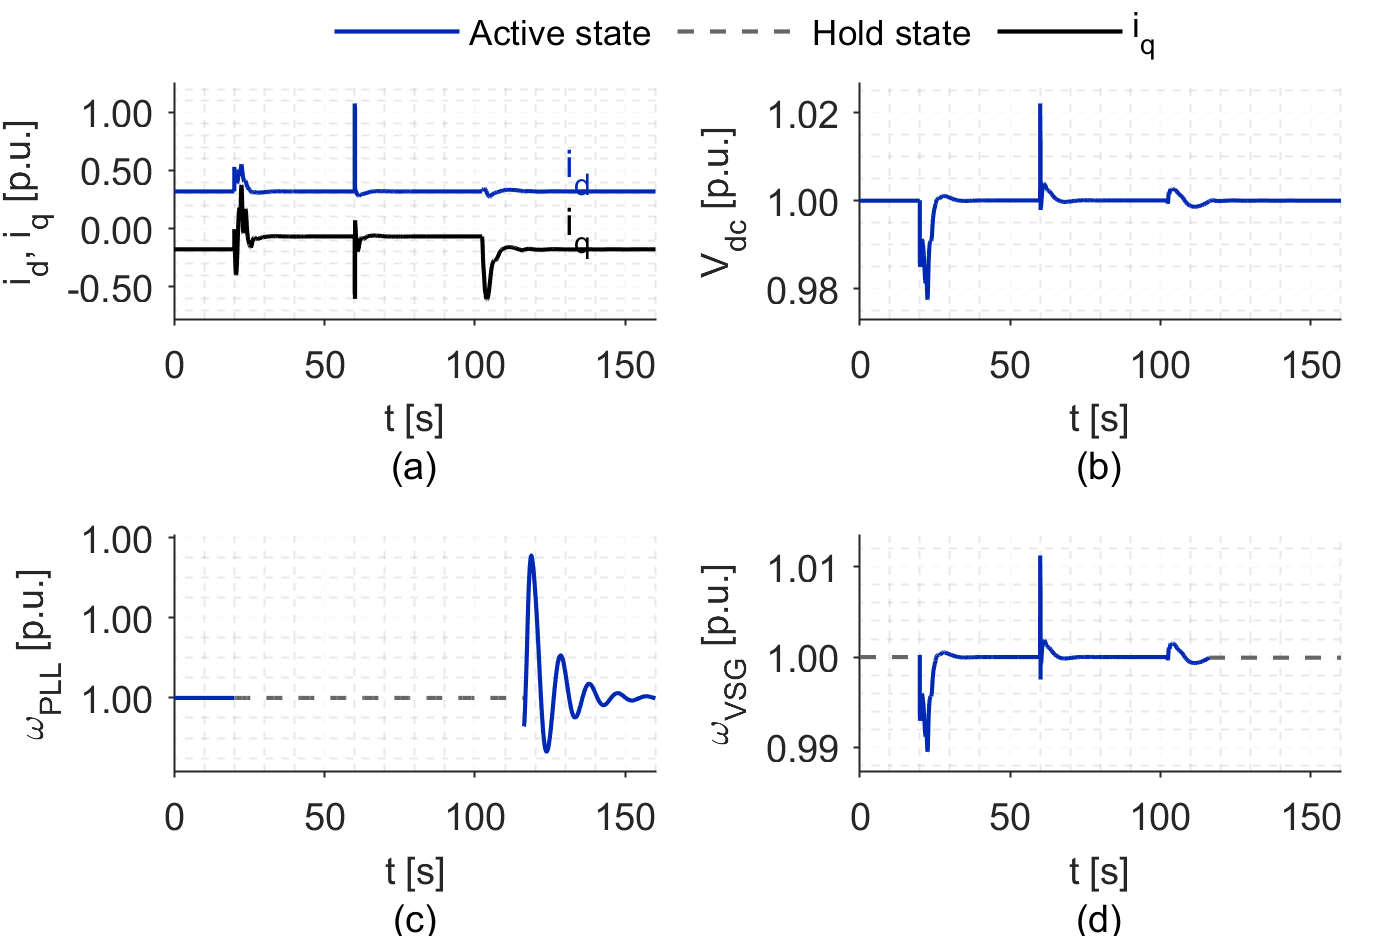
\includegraphics[width=0.46\textwidth]{sg_fault_cycle160_ibr_states_v15.png}
\captionof{figure}{สถานะของ IBR ในกรณีทดสอบ 160 s เส้นทึบคือสถานะของ branch ที่ทำงาน ส่วนเส้นประคือสถานะของ branch ที่ถูก hold}
\end{center}

{\small\textbf{อ่านกราฟอย่างไร:} ช่วงเหตุการณ์ที่ $t\approx20$, $60$ และ $100$ s มี transient ตามการรบกวน แต่ไม่เกิดการระเบิดของสถานะหรือการเริ่มต้นใหม่จากศูนย์ ส่วน $V_{dc}$ ยังอยู่ใกล้ $1\pu$ ตลอดการจำลอง}

\vfill
\warnbox{คำว่า ``bumpless'' ในงานนี้หมายถึงไม่มี jump ของปริมาณที่ขั้วต่อซึ่งฉีดเข้าสู่โครงข่าย ไม่ได้หมายความว่าสถานะภายใน controller ทุกตัวหรือพิกัด $dq$ ทุกแกนต้องมีค่าคงเดิม}
\clearpage

\sectitle{B2 ทำไมมี IBR 4 ตัว แต่สลับเพียงบางตัว}{Readiness check และการเลือกชุด GFM}

\answerbox{ค่า severity บอกเพียงว่า ``เมื่อไรระบบต้องการ GFM เพิ่ม'' แต่ไม่ได้บอกว่า ``IBR ตัวใดต้องสลับ'' การเลือกตัวสลับเป็นหน้าที่ของ selector ซึ่งพิจารณาเฉพาะ configuration ที่ตรวจสอบไว้แล้ว และเลือกชุดที่เพิ่ม GFM น้อยที่สุดแต่ยังผ่านเงื่อนไขของระบบ}

\vspace{5pt}
\begin{center}
\begin{tikzpicture}[font=\small,>=Latex,node distance=5mm and 5mm,
 box/.style={draw=navy,rounded corners=2pt,fill=lightblue,minimum height=9mm,text width=3.2cm,align=center},
 gate/.style={draw=blue,diamond,aspect=2.2,fill=lightyellow,text width=2.2cm,align=center},
 arr/.style={->,thick,draw=navy}]
\node[box] (measure) {คำนวณ $S_i$ จากแรงดันแต่ละบัสและ $f_{\mathrm{COI}}$};
\node[gate,right=of measure] (dwell) {$S_i\ge\Gamma_{on}$ ครบ dwell?};
\node[box,right=of dwell] (table) {ค้นหา strict superset ของชุด GFM ปัจจุบัน};
\node[box,below=of table] (check) {ตรวจ feasibility, KCL, ข้อจำกัดอุปกรณ์ และ SSSA};
\node[gate,left=of check] (pass) {candidate ผ่านทุกข้อ?};
\node[box,left=of pass] (rank) {จัดอันดับและเลือกชุดที่เปลี่ยนน้อยที่สุด};
\node[box,below=of rank] (commit) {commit แบบ atomic หรือคงโหมดเดิมถ้าไม่ผ่าน};
\draw[arr] (measure)--(dwell); \draw[arr] (dwell)--node[above]{ใช่}(table);
\draw[arr] (table)--(check); \draw[arr] (check)--(pass);
\draw[arr] (pass)--node[above]{ผ่าน}(rank); \draw[arr] (rank)--(commit);
\draw[arr] (dwell.south) |- node[pos=.25,right]{ไม่ใช่}(commit.east);
\draw[arr] (pass.south) |- node[pos=.25,right]{ไม่ผ่าน}(commit.east);
\end{tikzpicture}
\end{center}

\begin{minipage}[t]{0.49\textwidth}
\textbf{Readiness check ตรวจอะไร}
\begin{enumerate}
  \item จุดสมดุลของ configuration เป้าหมายต้องแก้ได้
  \item residual ของสมการโครงข่าย/KCL ต้องอยู่ใน tolerance
  \item เงื่อนไขอุปกรณ์และ short-circuit strength ต้องไม่ถูก veto
  \item ผล SSSA ของระบบเต็มต้องผ่านเกณฑ์ damping ที่กำหนด
  \item อุปกรณ์ที่จะเปลี่ยนโหมดต้องผ่าน hold/lockout และ transfer map
\end{enumerate}
\end{minipage}\hfill
\begin{minipage}[t]{0.49\textwidth}
\textbf{หลักการจัดอันดับ}
\begin{enumerate}
  \item ตัด candidate ที่ไม่ผ่านออกก่อน
  \item เพิ่มจำนวน GFM เท่าที่จำเป็น ไม่สลับทุกตัวพร้อมกัน
  \item ถ้าจำนวนเท่ากัน เลือก configuration ที่มี stability margin สูงกว่า
  \item ใช้ device ID เป็นตัวตัดสินกรณีคะแนนเท่ากัน เพื่อให้ผลทำซ้ำได้
\end{enumerate}
\end{minipage}

\vspace{5pt}
\noindent\colorbox{lightblue}{\parbox{\dimexpr\textwidth-2\fboxsep\relax}{\small\textbf{ตัวอย่างจากกรณีศึกษา:} หลัง SG trip ที่ $t=20$ s, IBR ที่บัส 2 รับหน้าที่ angle reference และเป็น GFM ก่อน ต่อมาที่ $t=22.089$ s selector เลือกชุดเป้าหมาย $\{$บัส 2, บัส 6$\}$ จึงมีเพียง IBR ที่บัส 6 ซึ่งต้องเปลี่ยนโหมดจริง การที่ severity ของบัสอื่นสูงไม่ได้แปลว่าบัสนั้นต้องถูกเลือก}}

\vspace{4pt}
\noindent\colorbox{lightgreen}{\parbox{\dimexpr\textwidth-2\fboxsep\relax}{\small\textbf{ถ้าต้องสลับพร้อมกันหลายตัว จะประสานกันอย่างไร?} ในกรณีศึกษานี้มี GFM สองตัวทำงานพร้อมกันจริง คือบัส 2 ช่วง $t=20$--$116$ s และบัส 6 ช่วง $t=22.089$--$25.303$ s การประสานกันไม่ได้ใช้ตัวควบคุม power sharing ส่วนกลาง แต่เกิดจากแต่ละตัวเป็นแหล่งจ่ายแรงดันที่มีพลวัตสวิงและการตอบสนอง $Q$--$V$ เป็นของตัวเอง แล้วแบ่งภาระกันผ่านโครงข่าย ตัวคุมมีค่าหน่วง $D_v$ ในสมการสวิงและค่าเกน $k_Q,k_E$ ในลูปแรงดัน ซึ่งทำหน้าที่คล้าย droop โดยธรรมชาติ}}

\vspace{4pt}
\noindent\colorbox{lightyellow}{\parbox{\dimexpr\textwidth-2\fboxsep\relax}{\small\textbf{เปรียบเทียบกับ Fixed GFM แล้วหรือไม่?} มีแล้ว งานนี้มีการศึกษาแบบหลาย arm บน chronology เดียวกัน โดยทุก arm เริ่มจาก base case ชุดเดียว แก้เฉพาะตัวเลือกที่เป็นนโยบาย ดังนั้นความต่างที่เห็นจึงมาจากนโยบาย ไม่ใช่จากเงื่อนไขตั้งต้น arm ประกอบด้วย adaptive ตามนโยบายที่ส่งมอบ, pinned GFM หนึ่งตัว, pinned GFM สองตัว, pinned GFM ทั้งสี่ตัว และ locked GFL ที่ตรึงเป็น GFL ทั้งหมด นอกจากนี้ยังมี arm กลุ่ม no-adaptation ที่เลือก GFM ครั้งเดียวตอน SG trip แล้วไม่ปรับอีก กรณี locked GFL ถูกกำหนดให้ล้มเหลวแบบ fail-closed ด้วยเหตุผลว่าไม่มีแหล่ง forming ในเกาะ และการศึกษาให้นับว่า arm ที่ล้มเหลวตรงตามที่คาดไว้ถือเป็นผลที่ถูกต้อง}}

\vspace{3pt}
\noindent\colorbox{lightyellow}{\parbox{\dimexpr\textwidth-2\fboxsep\relax}{\small\textbf{แล้วทำไมไม่เทียบกับวิธีในวรรณกรรม?} ตรงนี้เป็นข้อจำกัดจริง งานของ Ding et al. ถูกอ้างอิงในเชิงแนวคิดเรื่องการสลับโหมดและการรักษาความต่อเนื่องของ state แต่ไม่ได้ใช้เป็นคู่เปรียบเทียบเชิงตัวเลข จึงควรตอบว่า การเทียบกับวิธีสลับโหมดของงานอื่นยังไม่ได้ทำในงานนี้}}
\clearpage

\sectitle{B3 ค่า threshold และ dwell มาจากไหน}{Supervisor tuning และ $f_{\mathrm{COI}}$}

\answerbox{ค่าชุดนี้เป็นค่าที่เลือกใช้ในการศึกษากรณี IEEE 14-bus โดยออกแบบให้มี hysteresis และเวลายืนยันเหตุการณ์ ไม่ใช่ค่าที่พิสูจน์แล้วว่าเหมาะที่สุด จุดประสงค์คือให้ระบบตอบสนองเร็วเมื่อจำเป็นต้องเพิ่ม GFM แต่คืนสู่ GFL อย่างระมัดระวังเมื่อระบบฟื้นตัว}

\vspace{3pt}
\begin{minipage}[t]{0.52\textwidth}
ดัชนีที่ IBR ตัวที่ $i$ ใช้คือ
\[
J_{V,i}=\frac{|V_i-V_{i,\mathrm{healthy}}|}{0.10},\qquad
J_f=\frac{|f_{\mathrm{COI}}-60|}{0.50},
\]
\[
S_i=\operatorname{sat}\!\left(0.5J_{V,i}+0.5J_f\right),\qquad 0\le S_i\le1.
\]

\begin{center}
\small
\begin{tabularx}{\linewidth}{@{}>{\bfseries}l c X@{}}
\toprule
พารามิเตอร์ & ค่าที่ใช้ & เหตุผลทางวิศวกรรม \\
\midrule
$w_V,w_f$ & $0.5,0.5$ & ให้แรงดันเฉพาะบัสและความถี่รวมมีน้ำหนักเท่ากัน \\
$\Gamma_{on}$ & 0.65 & ขอ GFM เมื่อความรุนแรงสูงชัดเจน \\
$\Gamma_{off}$ & 0.35 & แยกจากค่า on เพื่อสร้าง hysteresis \\
$T_{d,on}$ & 0.10 s & กรอง spike สั้น แต่ยังตอบสนองได้เร็ว \\
$T_{d,off}$ & 1.00 s & ต้องเห็นการฟื้นตัวต่อเนื่องก่อนลด GFM \\
\bottomrule
\end{tabularx}
\end{center}
\end{minipage}\hfill
\begin{minipage}[t]{0.45\textwidth}
\textbf{ผลของ dwell ที่ควรเข้าใจ}
\begin{center}
\begin{tikzpicture}[x=0.65cm,y=0.7cm,font=\scriptsize]
\draw[->] (0,0)--(7.1,0) node[right]{$t$};
\draw[->] (0,0)--(0,3.3) node[above]{$S_i$};
\draw[dashed,gray] (0,1.8)--(7,1.8) node[right]{$\Gamma_{on}$};
\draw[blue,thick] plot[smooth] coordinates{(0,.7)(1,2.5)(1.7,1.4)(2.5,2.7)(4.6,2.4)(5.1,1.1)(7,.8)};
\draw[<->,red,thick] (1,2.9)--(1.7,2.9) node[midway,above]{สั้น};
\draw[<->,navy,thick] (2.5,3.15)--(4.6,3.15) node[midway,above]{ยาวพอ};
\end{tikzpicture}
\end{center}
\small
ถ้า dwell สั้นเกินไป spike แรกอาจทำให้สลับโดยไม่จำเป็นและเกิด chattering ได้ แต่ถ้ายาวเกินไป ระบบจะช้าเมื่อสูญเสียแหล่งอ้างอิง ค่าที่ใช้จึงเลือกแบบไม่สมมาตร: เพิ่ม support เร็วและถอน support ช้า

\textbf{ทำไมใช้ $f_{\mathrm{COI}}$}
\begin{itemize}
  \item เป็นค่าเฉลี่ยถ่วงน้ำหนักด้วยค่าคงที่ inertia $H$ ของอุปกรณ์ที่ \emph{มี} พลวัตความถี่ คือ SG และ GFM เท่านั้น ส่วน GFL ถูกตัดออกเพราะไม่มี inertia state
  \item ถ้าไม่มีอุปกรณ์ใดเข้าเกณฑ์ ค่าที่ได้จะเป็น NaN ไม่ใช่ศูนย์ ซึ่งทำให้ตรวจสอบย้อนหลังได้ว่าขณะนั้นคำนวณดัชนีไม่ได้
  \item IBR ทุกตัวใช้ $J_f$ ตัวเดียวกัน จึงไม่ตัดสินจาก PLL เฉพาะจุดซึ่งอาจแกว่งไม่ตรงกัน
  \item ยังคงใช้ $J_{V,i}$ ของแต่ละบัส เพื่อรักษาข้อมูลปัญหาเฉพาะพื้นที่
\end{itemize}
\end{minipage}

\noindent\colorbox{lightblue}{\parbox{\dimexpr\textwidth-2\fboxsep\relax}{\small\textbf{ผลจาก run 160 s:} $f_{\mathrm{COI}}$ อยู่ในช่วง 59.240--60.676 Hz และขนาดแรงดันต่ำสุดในระบบวัดได้ 0.258 pu ระหว่างฟอลต์ที่บัส 9}}

\vspace{3pt}
\noindent\colorbox{lightyellow}{\parbox{\dimexpr\textwidth-2\fboxsep\relax}{\small\textbf{ถ้ามี communication delay จะยังใช้ได้ไหม?} $T_{d,on}=0.10$ s เป็นเวลายืนยัน ไม่ใช่เวลาสื่อสาร ดังนั้นยิ่ง delay มาก เวลาที่ใช้ตัดสินใจจริงจะยิ่งยาวขึ้นและตอบสนองช้าลง จุดที่ต้องระวังคือถ้า delay ใกล้หรือเกิน 0.10 s ระบบจะตอบสนองช้ากว่าที่ออกแบบ ซึ่งงานนี้ \textbf{ยังไม่ได้จำลอง} จึงยังตอบแทนระบบจริงไม่ได้ แนวทางที่ควรพิจารณาในงานต่อไปคือใช้ความถี่เฉพาะพื้นที่ (local frequency) เป็นเงื่อนไขสำรอง เพื่อให้ตัดสินใจได้โดยไม่ต้องรอข้อมูลจากส่วนกลาง หรือเพิ่มเวลาเผื่อสำหรับ delay ไว้ใน dwell}}

\vfill
\warnbox{โครงการนี้ยังไม่มี sensitivity sweep จึงควรตอบว่าค่าพารามิเตอร์ ``มีเหตุผลรองรับและใช้ได้กับกรณีศึกษานี้'' ไม่ควรตอบว่าเป็นค่าที่เหมาะที่สุด}
\clearpage

\sectitle{B4--B7 คำถามต่อยอดที่ควรตอบให้ชัด}{Controller, fault ride-through, การคืนโหมด และ stability}

\begin{minipage}[t]{0.475\textwidth}
\noindent\colorbox{lightblue}{\parbox{\dimexpr\linewidth-2\fboxsep\relax}{\textbf{B4: state ของ branch ที่ไม่ได้ทำงานไปอยู่ที่ไหน?}}}

แบบจำลองใช้ state vector ขนาดคงที่ซึ่งมี plant ร่วมและ controller สอง branch
\[
\underbrace{[i_d,i_q,V_{dc},I_{dc}]}_{\text{shared plant}}
\oplus\underbrace{x_{GFL}}_{\text{PLL, P/Q, current loops}}
\oplus\underbrace{x_{GFM}}_{\text{VSG, voltage/current loops}}.
\]
เมื่ออยู่โหมด GFL จะคำนวณอนุพันธ์เฉพาะ shared plant และ $x_{GFL}$ ส่วน $x_{GFM}$ ถูก hold ไว้; เมื่อเป็น GFM จะสลับกัน ก่อนเปิดใช้ branch ใหม่จะ initialize จาก $V,I,P,Q$ ที่ขั้วต่อจริง จึงไม่ดึงค่าเก่าที่ไม่สอดคล้องกลับมาใช้งาน

\smallskip
\textbf{เรื่อง PLL ตอน fault:} ในโหมด GFM ไม่มี PLL เป็นตัวกำหนดมุม เพราะมุมมาจาก VSG ส่วนในโหมด GFL PLL ยังเป็น active state ดังนั้นงานนี้ไม่ควรอ้างว่า PLL ``ไม่มีวันหลุดล็อก'' แต่ควรพิจารณาจาก trajectory และเงื่อนไขการสลับของกรณีทดสอบ

\medskip
\noindent\colorbox{lightyellow}{\parbox{\dimexpr\linewidth-2\fboxsep\relax}{\textbf{B6: กลับจาก GFM เป็น GFL อย่างไร?}}}

หลัง SG ถูกเสนอให้กลับเข้าระบบที่ $t=100$ s จะยังไม่ปิดทันที ต้องผ่าน synchronism guard ก่อน และ reclose สำเร็จที่ $t=102.363$ s จากนั้น
\begin{itemize}
  \item $T_{hold}=1.0$ s ป้องกันการเปลี่ยนซ้ำทันทีหลังเหตุการณ์
  \item $T_{lock}=2.0$ s ป้องกันคำสั่งย้อนกลับในช่วงที่ transient ยังไม่จบ
  \item เมื่อ severity ต่ำกว่า $\Gamma_{off}$ ต่อเนื่องตาม dwell และไม่มี timer ขวาง จึง hand back reference ให้ SG และคืน IBR เป็น GFL
\end{itemize}
ใน run นี้ IBR หลักคืนเป็น GFL ที่ $t=116.238$ s จึงไม่ได้รีบคืนโหมดทันทีที่ SG reclose

\medskip
\noindent\colorbox{lightblue}{\parbox{\dimexpr\linewidth-2\fboxsep\relax}{\textbf{B8: มีอะไรรับประกันว่าไม่ singular และขยายระบบใหญ่ได้ไหม?}}}

\textbf{การรับประกันเท่าที่มี}
\begin{itemize}
  \item ก่อน commit ทุกครั้ง ต้องมีจุดสมดุลที่ผ่านการรับรอง พร้อม input ที่รับรองคู่กับ configuration นั้น ถ้าไม่มีจะปฏิเสธทันที (ข้อความในโค้ดคือ ``refusing to commit an uncertified operating point'')
  \item ถ้าเกาะใดไม่มีแหล่ง voltage-forming เหลืออยู่ ระบบหยุดแบบ fail-closed ด้วยเหตุ \texttt{noVoltageFormingSource} และไม่ส่งเข้าตัวแก้สมการ
  \item ถ้าคำตอบฝั่งขวาของเหตุการณ์แก้ไม่ลู่เข้า จะนับเป็นการปฏิเสธ ไม่ใช่การยอมรับ พร้อมหน่วงเวลาก่อนลองใหม่
  \item มีการตรวจสภาพเงื่อนไขของเมทริกซ์ (rcond) ทั้งใน SSSA และการแก้จุดสมดุล ถ้าต่ำกว่าเกณฑ์ที่กำหนดจะล้มเหลวแบบปิด
  \item ขั้นเวลาจะถูกหดลงต่ำสุดหลังพบ discontinuity และถ้ายังแก้ไม่ได้จะลองวิธี implicit order ต่ำลง แต่ \textbf{ไม่มีการลดระดับไปใช้ fixed step อย่างเงียบ ๆ}
\end{itemize}

\textbf{Scalability} ปัจจุบันตรวจสอบบน IEEE 14-bus เท่านั้น การขยายไป New England 39-bus ถูกบันทึกไว้ในแผนของเครื่องมือ SSSA แต่ยังไม่ได้ทำ คอขวดแรกที่คาดว่าจะเจอคือจำนวน configuration ที่ต้องตรวจรับรองล่วงหน้า ซึ่งเพิ่มขึ้นตามจำนวนชุด GFM ที่เป็นไปได้ จึงต้องแก้ทั้งต้นทุนการรับรองและการจัดเก็บตาราง ก่อนจะไปถึงเรื่องการประสานกันของ GFM จำนวนมาก
\end{minipage}\hfill
\begin{minipage}[t]{0.475\textwidth}
\noindent\colorbox{lightred}{\parbox{\dimexpr\linewidth-2\fboxsep\relax}{\textbf{B5: จำกัดกระแสด้วยวิธีใด และยังคุมเสถียรภาพอย่างไร?}}}

วิธีที่ใช้คือ \textbf{circular clamp บนเวกเตอร์กระแสอ้างอิง} คือถ้าขนาดเกิน $I_{max}$ จะย่อเวกเตอร์ลงโดยรักษาทิศทางไว้
\[
r=\left\|\mathbf{i}_{ref}\right\|,\qquad
\mathbf{i}_{ref}\leftarrow\frac{I_{max}}{r}\,\mathbf{i}_{ref}\quad (r>I_{max}).
\]
แบบจำลองนี้ \textbf{ไม่ใช้ virtual impedance} (มีคอมเมนต์กำกับไว้ในโมเดลโดยตรง) และไม่ตัดกระแสจริงแบบทันทีทันใด แต่ใช้ anti-windup แบบ conditional hold คือ \emph{หยุด} อินทิเกรตของลูปแรงดันเมื่อ limiter ทำงานและอินทิเกรตอร์กำลังดันเข้าไปในลิมิตมากขึ้น

\textbf{ทำไมยังไม่เสีย synchronism}

สมการสวิงของ VSG ที่กำหนดความถี่และมุมยังทำงานตามปกติ ขณะที่ถูกจำกัดคือเฉพาะเวกเตอร์กระแสอ้างอิง ดังนั้น converter จึงยังคงพฤติกรรมเป็นแหล่งจ่ายแรงดันอยู่ และมุมยังถูกกำหนดโดยพลวัตของ VSG ไม่ได้ถูกแช่แข็งพร้อมกับกระแส

\centering
\includegraphics[width=\linewidth,height=5.0cm,keepaspectratio]{backup_b5_fault_current.png}
\captionof{figure}{กระแส IBR และแรงดันบัส 9 ระหว่าง fault 150 ms}
\raggedright\small

\textbf{แล้วค่า $P$ ที่ขึ้นไป 2.17 pu ล่ะ?} ค่าสูงสุดของ $P$ เกิดที่ $t=60.150$ s ซึ่งเป็น sample เดียวกับที่ $|V|$ ที่บัสนั้นพุ่งเป็น 1.86 pu ขณะเคลียร์ฟอลต์ อัตราส่วน $P/|V|\approx1.17$ pu จึงยังสอดคล้องกับกระแสที่ถูกจำกัด ไม่ได้หมายความว่ากระแสทะลุ $1.20\pu$ การที่ $P$ ดูเกินพิกัดเป็นผลจากแรงดันที่พุ่งชั่วขณะ ไม่ใช่กระแสที่เกินพิกัด

สำหรับกระแสจริง ขีดจำกัด $1.20\pu$ และกระแสที่รายงานอยู่ใน\textbf{ฐานเดียวกัน} และค่าสูงสุดที่วัดได้จากผลการจำลองคือ $1.2140\pu$ ที่ $t=60.0109$ s ซึ่งเกินเส้นอ้างอิงอยู่เล็กน้อยในระดับเสี้ยววินาที ไม่ใช่ค่าคงตัวตลอดช่วงฟอลต์

\medskip
\noindent\colorbox{lightgreen}{\parbox{\dimexpr\linewidth-2\fboxsep\relax}{\textbf{B7: พิสูจน์ stability ของ switched system แล้วหรือยัง?}}}

\textbf{สิ่งที่งานนี้รองรับ}
\begin{itemize}
  \item ทุก configuration เป้าหมายผ่าน equilibrium/KCL และ full-order SSSA ก่อนถูกเลือก
  \item transfer map ตรวจ continuity ของกระแสก่อน commit
  \item กรณีทดสอบ 160 s ซึ่งมี SG trip, fault, reclose และ handback จำลองจบโดย trajectory ไม่ลู่ออก
\end{itemize}
\textbf{สิ่งที่ยังไม่ได้พิสูจน์}
\begin{itemize}
  \item ยังไม่มี global stability proof ของ hybrid DAE ทุกลำดับการสลับ
  \item ยังไม่มี multiple-Lyapunov หรือ average dwell-time certificate
  \item ยังไม่ได้ทดสอบ robustness ต่อ measurement noise, delay และการเปลี่ยน tuning เป็นช่วงกว้าง
\end{itemize}
ดังนั้นข้อสรุปที่ถูกต้องคือ ``ผ่านการตรวจระดับ configuration และผ่านกรณีศึกษาที่กำหนด'' ไม่ใช่ ``เสถียรสำหรับ disturbance ทุกชนิด''
\end{minipage}

\vfill
\answerbox{ภาพรวมของแนวทางนี้คือ: วัดความรุนแรงเพื่อบอกจังหวะ เลือก configuration จากชุดที่ตรวจไว้ สลับด้วย transfer map ที่รักษาปริมาณขั้วต่อ และใช้ hysteresis/dwell/hold/lockout เพื่อไม่ให้เปลี่ยนโหมดถี่เกินไป}

\end{document}
